
\section{Ziel}
In diesem Versuch soll der glühelektrische Effekt in Abhängigkeit der Temperatur untersucht werden.
\section{Theorie}
\subsection{Austrittsarbeit und Richardson-Gleichung}
Metalle weisen in der Regel eine Kristallstruktur auf, aufgrund derer sie eine hohe elektrische Leitfähigkeit aufweisen. Diese rührt daher, dass die Atome im Kristallgitter fast alle ausnahmslos ionisiert vorliegen, sodass sich
in deren gemeinsamen Kraftfeld Elektronen frei bewegen können, die sogenannten Leitelektronen.
Da das durch die Ladungen verursachte Gitterpotential an den Gitterpunkten hohe Werte annimmt, abseits dieser jedoch nahezu unverändert ist, kann dieses grob als konstant genähert werden.
Somit befindet sich innerhalb des Metalls ein postives Gitterpotential , welches sich durch den Betrag $\phi$ vom äußeren Potential unterscheidet. Es liegt ein sogenannter Potentialtopf vor, der in Abbildung \ref{fig:pt} dargestellt ist.
\begin{figure}[H]
  \centering
  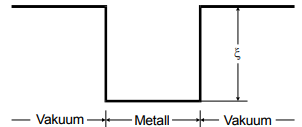
\includegraphics{Text/Bilder/Potentialtopf.png}
  \caption{Darstellung eines Potentialtopfs \cite[93]{sample}}
  \label{fig:pt}
\end{figure}
Wenn ein Elektron dieses Potentialtopf verlassen will, muss dieses die Austrittsarbeit $e_0 \zeta$ aufbringen. Dabei ist $e_0$ die Elementarladung und $\zeta$ die fermische Grenzenergie.
Letztere gibt die Maximalenergie der Elektronen bei $T=0$ in Abhängigkeit der Elektronendichte an. Ebenso gilt bei Raumtemperatur $\zeta \gg kT$.
Auf die Frage ob ein Elektron die Metalloberfläche spontan verlassen kann, gibt die Quantenmechanik folgende Einschränkungen:
\begin{itemize}
\item Elektronen können nur diskrete Energiewerte annehmen
\item Die Elektronen unterliegen in diesem Fall dem Pauli-Verbot, das heißt, dass jeder Energiezustand nur mit 2 Elektronen mit entgegengesetzten Spin besetzt werden kann.
\end{itemize}
Daraus folgt, dass Elektronen auch beim absoluten Nullpunkt eine endliche Energie aufweisen.
Wie wahrscheinlich es ist, dass ein Energiezustand im thermische Gleichgewicht besetzt wird, gibt die Fermi-Diracsche Verteilungs-Funktion \eqref{eqn:FDV} an.
\begin{equation}
  f(E)=\frac{1}{\exp{\left(\frac{E-\zeta}{kT}\right)+1}} \label{eqn:FDV}
\end{equation}
Der Kurvenverlauf ist ein Abbildung \ref{fig:KVL} zu sehen.
\begin{figure}[H]
  \includegraphics{Text/Bilder/kurvenverlauf.png}
  \caption{Der Verlauf der Fermi-Diracschen Verteilungsfunktion am absoluten Nullpunkt (durchgezogene
Linie) und bei T >> 0 (gestrichelte Linie) \cite[94]{sample} }
  \label{fig:KVL}
\end{figure}
Es ist zu erkennen, dass eine Energie von $\zeta+e_0 \phi$ nötig ist, damit ein Elektron die Metalloberfläche verlassen kann. Experimentelle Beobachtungen haben ergeben, dass für so einen Fall auch beim Schmelzpunkt von Wolfram noch
$e_0 \phi \gg kT$ gilt, weshalb \eqref{eqn:FDV} genähert werden kann:
\begin{equation}
    f(E) \approx \exp{\left(\frac{\zeta-E}{kT}\right)}
\end{equation}
Die Menge der Elektronen $d\alpha$ aus dem Volumenelement des Impulsraums wird durch
\begin{equation}
  d \alpha = v_z n(E) dp_x dp_y dp_z \label{eqn:dalpha}
\end{equation}
\begin{center}
 \tiny {($v_z=\text{Geschwindigkeit der Elektronen zur Oberflächennormalen}$,  $n(E)=\frac{2}{h^{3}}f(E)$)}
\end{center}
beschrieben. Mithilfe der kinetischen Energie kann mit \eqref{eqn:dalpha} die Richardson-Gleichung hergeleitet werden:
\begin{equation}
   	J_\text{S} =  \frac{4 \pi e_0 m_0 k^2}{h^3} T^2 \exp\left(-e_0 \frac{\phi}{k T}\right)\text{.} \label{eq:Richardson-Gleichung}
\end{equation}
\begin{center}
 \tiny {($h=\text{Planck'sches Wirkungsquantum}$)}
\end{center}
Diese beschreibt die Stromdichte der austretenden Elektronen.

\subsection {Hochvakuum-Diode}
Da Elektronen mit Gasen in der Luft wechselwirken können und dies die Messungen verfälschen könnte, wird der Sättigungsstrom im Hochvakuum gemessen.
Ebenso werden die Elektronen nach Austritt aus der Metalloberfläche mithilfe des elektrischen Feldes einer Anode abgesogen. Die Hochvakuum-Diode ist in Abbildung \ref{fig:Hochvakuum-Diode} dargestellt.
\begin{figure}[H]
  \centering
  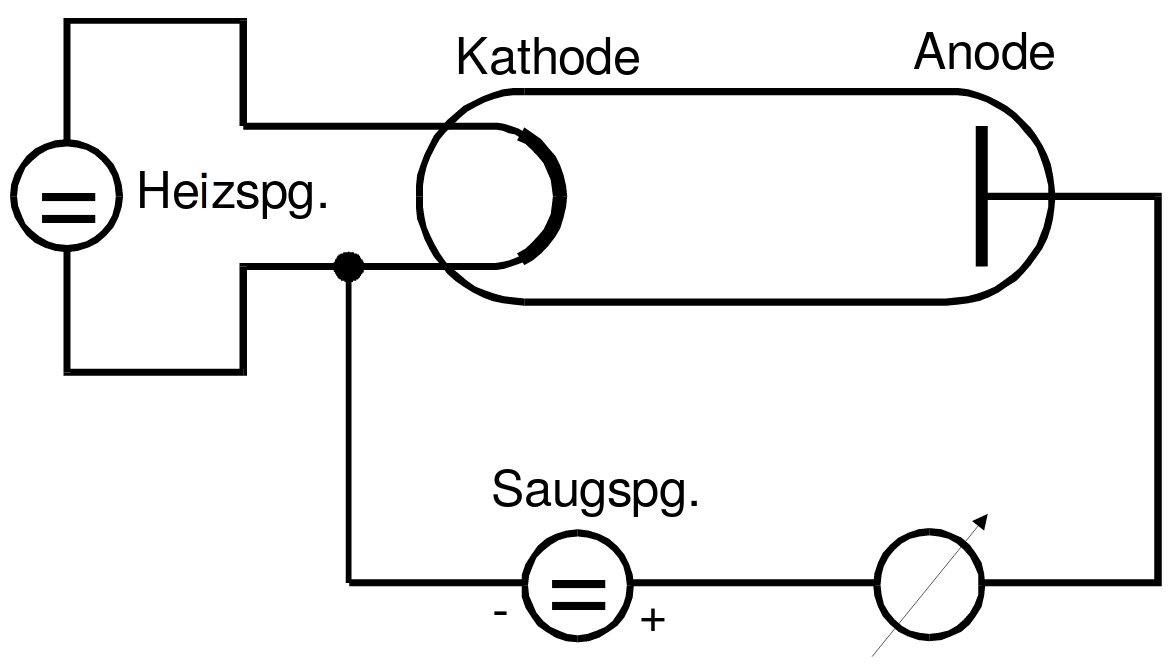
\includegraphics[scale=0.25]{Text/Bilder/Hochvakuum-Diode}
  \caption{Grundsätzliche Beschaltung einer Hochvakuum-Diode \cite[96]{sample}}
  \label{fig:Hochvakuum-Diode}
\end{figure}

\subsection{Die Langmuir-Schottkysche Raumladungsgleichung }
Elektronen werden zur Anode hin beschleunigt, wodurch die Geschwindigkeit $v$ der Elektronen nicht konstant ist.
Daher folgt aus $I=\rho v=\text{const.}$, dass die Raumladungsdichte $\rho$ zur Anode hin abnehmen muss.
Aufgrund der hohen Raumladung an der Kathode erreichen die Feldlinien der Anode nicht alle austretenden Elektronen, weshalb der gemessene Diodenstrom kleiner als der zu erwartende Sättigungsstrom ist.
Die Stromstärke innerhalb des Raumladungsgebiets lässt sich durch die Langmuir-Schottkysche Raumladungsgleichung \eqref{eqn:LSR}  beschreiben:
\begin{equation}
	J = \frac{4}{9} \epsilon_0 \sqrt{\frac{2 e_0^3 V^3}{a^4 m_0} } \label{eqn:LSR}
\end{equation}

\begin{center}
 \tiny {($v_z=\text{a=Abstand von Anode und Kathode}$)}
\end{center}

\subsection{Das Anlaufstromgebiet einer Hochvakuumdiode}
Die Gleichung \eqref{eqn:LSR} deutet an, dass $j=0$ ist, wenn keine Spannung anliegt. Jedoch ist auch in so einem Fall noch eine geringe Stromdichte messbar.
Dies lässt sich dadurch erklären, dass Elektronen eine größere Geschwindigkeit zur Oberflächennormalen haben können, als für den Austritt nötig wäre.
Somit besitzen solche Elektronen noch eine Restgeschwindigkeit, wenn sie aus dem Leiter austreten.
Wie groß die Anlaufstromstärke sein muss, damit ein Elektron die Anode noch erreicht, hängt von der Gegenspannung ab:
\begin{equation}
  J = J_0 \exp\left(-\frac{e_0 (-V +\phi_A)}{k T}\right)\text{.} \label{eqn:Anlaufstromstärke}
\end{equation}

\subsection{Kennlinie der Hochvakuum-Diode}
Als Kennlinie einer Hochvakuum-Diode wird der Zusammenhang zwischen Stromdichte $j$ und dem vom außen angelegten Potential bezeichnet.
Die Kennlinie kann in drei Bereiche unterteilt werden. Im ersten Bereich liegt eine Gegenspannung ($V<0$) an und es wird Anlaufstromgebiet genannt. In diesem ist ein exponentieller Anstieg erkennbar.
Der darauf folgende Bereich, das Raumladungsgebiet, zeichnet sich durch $ j \sim V^{\frac{3}{2}}$ aus, während das anschließende Sättigungsstromgebiet sich asymptotisch der
Sättigungsstromstärke $I_S$ annähert.
Ein schmematischer Kurvenverlauf ist ist Abbildung ist in \ref{fig:KHD} dargestellt.
\begin{figure}[H]
  \centering
  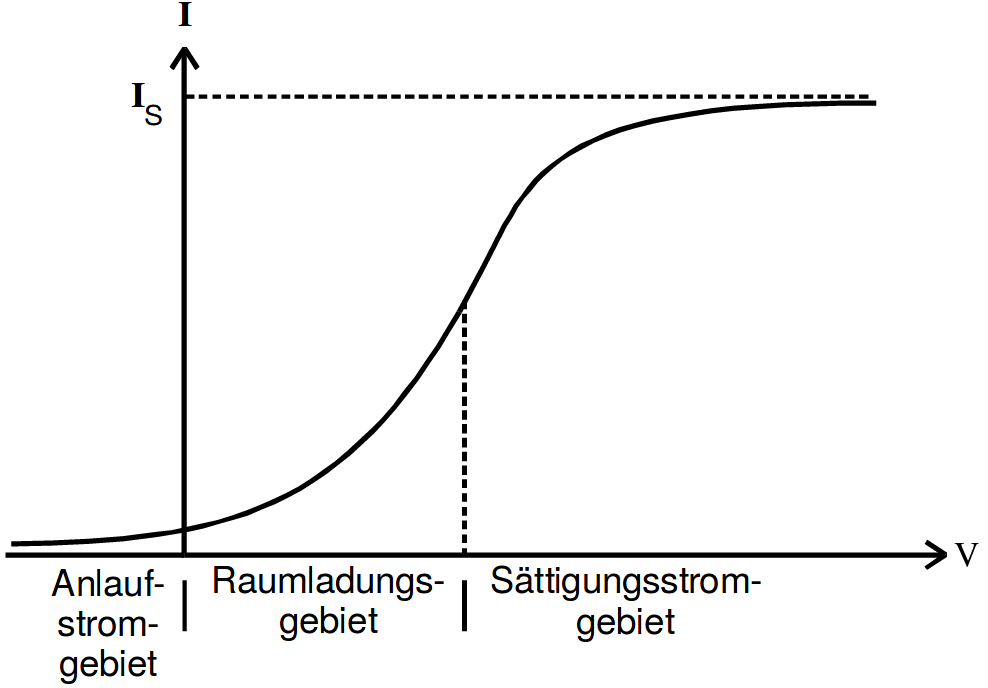
\includegraphics[scale=0.35]{Text/Bilder/Kennlinie.png}
  \caption{Kennlinie einer Hochvakuumdiode \cite[100]{sample}}
  \label{fig:KHD}
\end{figure}
